\chapter{Final System Design and Implementation}
\label{chap:implementation}

\begin{chapterplan}{15--18 pages}{Describe the archived repository, connect operational claims to code, and distinguish the active request paths from components that are present but not connected. Historical rationale is discussed in \cref{chap:evolution}.}
The implementation account is aligned with the hybrid-preferred production route after commit \texttt{5089fcc}. Snapshot \texttt{cb041d5} is retained only as the earlier dense-only inspection baseline. Values that were not preserved with the July evaluation are left unavailable rather than reconstructed from assumption.
\end{chapterplan}

\section{Chapter Scope and Evidence Basis}
\label{sec:implementation-scope}

The archived repository is the main evidence for this chapter. I inspected route handlers, schemas, services, frontend components, tests, configuration, and bundled data together because the presence of a file says little about whether a user-facing endpoint calls it. When documentation and the executable call graph disagree, the call graph is used to describe runtime behaviour.

Two modes are exposed through the shared Next.js/FastAPI shell. Document mode accepts PDFs, retrieves text and figures, and generates an answer. The 3D mode resolves an anatomy label and invokes export tools through an MCP stdio session. Their sources and evidence differ. Several advanced RAG modules remain present but are not connected to \codepath{/rag/ask}---notably post-generation citation filtering with a hard three-source limit and an effective \codepath{allow_world_knowledge} request field. I describe those as code assets without assigning production results to them.

\section{Final System Context and Deployment Topology}
\label{sec:final-system-context}

\begin{figure}[htbp]
  \centering
  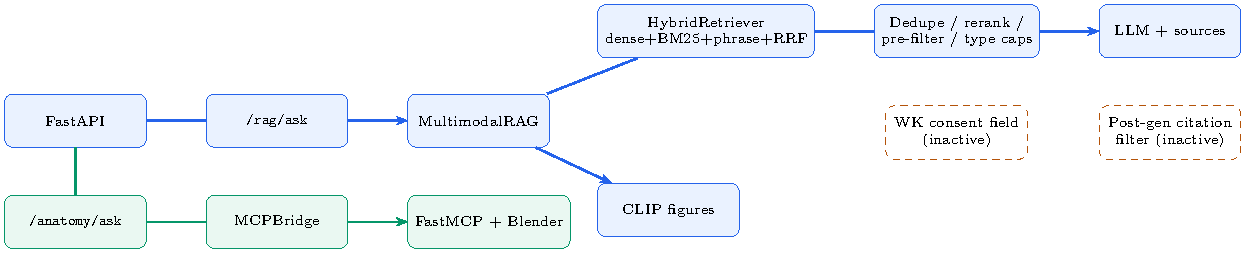
\includegraphics[width=\textwidth,height=0.70\textheight,keepaspectratio]{figures/rendered/final_runtime_architecture.pdf}
  \caption{Code-verified runtime architecture. Active hybrid retrieval stages are shown on the document path. The red block identifies controls that exist in the repository but are not effective on the production \codepath{/rag/ask} request path (notably world-knowledge consent and post-generation citation filtering).}
  \label{fig:final-runtime-architecture}
\end{figure}

The browser interface lives under \codepath{frontend/} and uses Next.js. Its main page contains the document chat, PDF upload controls, and a separate \codepath{AnatomyMcpPanel}. The browser defaults to \codepath{http://127.0.0.1:8000}, whereas the backend image exposes port \texttt{7860}; the frontend is also absent from \codepath{docker-compose.yml}. Deployment therefore requires an explicit API base and port mapping.

FastAPI composition occurs in \codepath{app/main.py}. The file registers ingestion, document-question, experiment, image, storage, visualisation, annotation, legacy Blender, and MCP anatomy routes. It also mounts local figures at \codepath{/outputs}, 3D files at \codepath{/anatomy-exports}, and the Three.js viewer at \codepath{/anatomy-viewer}. CORS origins come from \codepath{ALLOWED_ORIGINS}, with local and hosted defaults.

On the document side, uploads update the text and image indexes before the singleton \codepath{MultimodalRAG} is reloaded. A question then passes through MiniLM--Chroma retrieval, CLIP search, Groq generation, and an optional fixed-asset preview worker. That worker is a legacy HTTP service, not the Z-Anatomy MCP exporter. The 3D route launches \codepath{anatomy_mcp/server.py} as a child process, uses stdio, resolves catalogue entries, invokes Blender after a cache miss, and returns GLB and annotation URLs. This implements MCP's host--client--server separation \parencite{mcp20250618}.

The archive contains two different deployment arrangements. Local MCP operation expects Blender and Z-Anatomy \codepath{Startup.blend} outside the repository. The Compose stack supplies MinIO, the backend, and an older Blender HTTP worker based on \codepath{src/mcp/server.py}; it lacks both the FastMCP Z-Anatomy server and the source blend file. The Compose files therefore document storage and legacy previews rather than a complete containerised MCP deployment.

\section{Repository Structure and Responsibility Mapping}
\label{sec:repository-structure}

\Cref{tab:component-code-map} links each main responsibility to the files that implement it. The final column records what repository inspection established, including components that are not called by the production route.

\begin{table}[htbp]
  \centering
  \small
  \caption{Component-to-code mapping in the frozen repository.}
  \label{tab:component-code-map}
  \begin{tabularx}{\textwidth}{L{0.25\textwidth}L{0.34\textwidth}Y}
    \toprule
    Component & Main location & Verified role \\
    \midrule
    FastAPI composition & \codepath{app/main.py} & Routers, CORS, and static mounts. \\
    Document API & \codepath{app/api/routes/rag.py} & Exposes \codepath{POST /rag/ask}; forwards only \codepath{question}. \\
    Ingestion service & \codepath{app/services/ingestion_service.py} & Saves a PDF, runs text/image ingestion, rebuilds the image index, and reloads RAG. \\
    Text loading & \codepath{src/ingestion/loader.py} & PyMuPDF page loading, page heuristics, and chunking. \\
    Text store & \codepath{src/retrieval/vector_store.py} & Opens the MiniLM-backed Chroma collection under \codepath{processed/chroma}. \\
    Production RAG & \codepath{src/multimodal/multimodal_rag_chain.py} & Hybrid-preferred retrieval, rewrite, dedupe, rerank, pre-filter, type-dependent caps, synthesis, image reranking, grounding metadata. \\
    Hybrid retrieval & \codepath{src/retrieval/hybrid_retriever.py} & BM25, dense, phrase, and RRF; constructed by \codepath{MultimodalRAG}; dense fallback on failure. \\
    Figure pipeline & \codepath{src/ingestion/image_extractor.py}; \codepath{src/multimodal/multimodal_indexer.py} & Embedded-image extraction and complete CLIP-index rebuild. \\
    Storage & \codepath{app/services/object_storage.py} & MinIO/Supabase upload, signed URLs, and diagnostics. \\
    MCP REST layer & \codepath{app/api/routes/anatomy_mcp.py} & Health, search, ask, and export routes. \\
    MCP host/client & \codepath{app/services/anatomy_mcp_chat.py}; \codepath{app/services/anatomy_mcp_client.py} & Fast path, LLM tool loop, stdio session, tool discovery, and tool calls. \\
    MCP server & \codepath{anatomy_mcp/server.py} & Catalogue search, part export, and package export tools. \\
    Catalogue & \codepath{anatomy_mcp/label_index/exportable_catalog.json} & Geometry-probed structure entries. \\
    Blender scripts & \codepath{anatomy_mcp/blender_scripts/} & Z-Anatomy selection, GLB export, annotations, packages, and previews. \\
    Viewer & \codepath{anatomy_mcp/viewer/} & Three.js GLB loading and label display. \\
    \bottomrule
  \end{tabularx}
\end{table}

\section{Next.js Frontend and FastAPI API Layer}
\label{sec:frontend-api}

\subsection{Document Chat and Upload Interface}
\label{subsec:document-ui}

The main page holds the current conversation in browser state. Questions are posted to \codepath{/rag/ask}; PDFs use multipart upload to \codepath{/upload-pdf/}. The renderer can show answer text, source cards, and optional figures. When metadata are present, each source card includes a filename, page, and passage preview.

The frontend also sends \codepath{language} and \codepath{allow_world_knowledge} and displays states for consent and confidence. The frozen backend contract does not support that behaviour: \codepath{AskRequest} contains only \codepath{question}, and the route forwards \codepath{req.question}. Pydantic may ignore the extra fields, but they cannot change the request path. Several response fields expected by the browser are absent from \codepath{AskResponse} as well. For this snapshot, language choice, consent, confidence, and question-type handling are UI intentions rather than active backend controls.

\subsection{MCP Anatomy Interface}
\label{subsec:mcp-ui}

\codepath{AnatomyMcpPanel.js} sends the message and language to \codepath{/anatomy/ask}. Structured success data are handed to \codepath{AnatomyExportPanel}, which creates an iframe only when \codepath{anatomy_export.status == "ok"}. Ordinary errors therefore do not produce an empty viewer.

A compatibility function, \codepath{salvageExportFromAnswer}, searches assistant text for export URLs when structured data are missing. It supports older responses but weakens the verification contract because text-derived URLs may be stale, malformed, or unrelated to a completed tool call. Evaluation should either disable this path or record salvage-only cases separately.

\subsection{FastAPI Composition and Static Serving}
\label{subsec:fastapi-composition}

Route files parse requests and delegate to service modules. RAG uses \codepath{rag_service.py}, ingestion uses \codepath{ingestion_service.py}, storage uses \codepath{object_storage.py}, and anatomy requests pass to the MCP host. Generated files stay outside the frontend project; the backend exposes the relevant directories through static mounts and returns loadable URLs.

\section{PDF Ingestion, Cleaning, Chunking, and Metadata}
\label{sec:pdf-ingestion}

\codepath{upload_pdf} checks the file extension, writes the PDF to the raw-data directory, and performs a storage preflight. Text ingestion, image extraction, multimodal indexing, and \codepath{reload_rag} then run in sequence. The API response records status and elapsed time for each stage, so a partial failure remains visible.

The text loader scans every PDF in the raw directory with \codepath{PyMuPDFLoader}. It applies three inexpensive heuristics for likely index, contents, and glossary pages: an early ``index'' token, dotted chapter headings, and short comma-dense pages. These checks remove obvious noise but may also discard valid anatomy material. They are project-specific heuristics, not general PDF-cleaning guarantees.

Retained pages are divided by \codepath{RecursiveCharacterTextSplitter} into 800-character chunks with 150 characters of overlap. Fragments below 200 characters and dotted contents-like text are removed. Source and page metadata survive the split. The system embeds text with \codepath{sentence-transformers/all-MiniLM-L6-v2} \parencite{reimers2019,minilmModelCard} and appends records to collection \codepath{multimodal_rag} under \codepath{processed/chroma}.

Text indexing is append-oriented: the collection is not cleared, and stable identifiers are not derived from file and chunk hashes. Re-running ingestion over the same directory can create duplicate vectors. Retrieval-time filtering reduces repeated source cards without cleaning the store. A reproducible run should rebuild the collection from a clean, versioned corpus manifest.

Image ingestion behaves differently. Embedded raster images are enumerated, written locally, and stored with source, page, context, dimensions, and an object key. The service attempts upload to the configured object store, after which the multimodal index is cleared and rebuilt from valid metadata. Text and image indexes therefore have different update semantics.

\section{Text Retrieval: Hybrid-Preferred Production Route}
\label{sec:text-retrieval}

\subsection{Active Production Retrieval}
\label{subsec:active-text-retrieval}

\Cref{fig:rag-runtime-sequence} shows the active document path. \codepath{MultimodalRAG} constructs \codepath{HybridRetriever} once at initialisation and caches the BM25 index on disk. For each question it classifies the type, rewrites query variants, and requests hybrid candidates (dense, BM25, and phrase) with Reciprocal Rank Fusion defaults of 0.5, 0.4, and 0.1 and RRF constant 60 \parencite{karpukhin2020,robertson2009,cormack2009,reimers2019}. Candidate pools use up to 40 documents per query variant and a fused final pool of 32 before deduplication and reranking. If hybrid construction or search fails, the chain falls back to dense Chroma \codepath{similarity\_search}.

\begin{figure}[htbp]
  \centering
  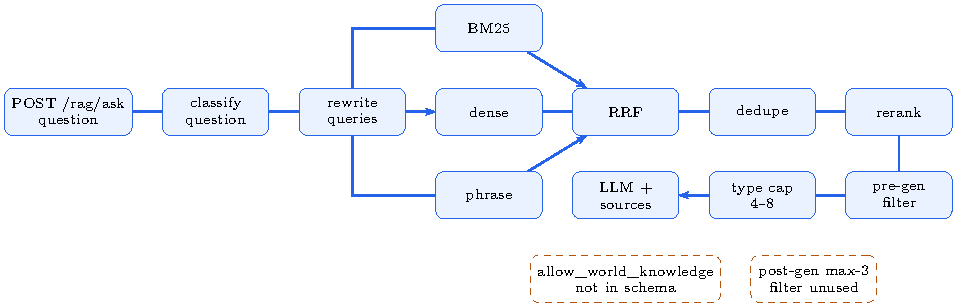
\includegraphics[width=\textwidth,height=0.68\textheight,keepaspectratio]{figures/rendered/rag_runtime_sequence.pdf}
  \caption{Production document request sequence after hybrid connection. Dashed orange notes identify repository controls that are not effective on this route (world-knowledge consent field; post-generation citation filter).}
  \label{fig:rag-runtime-sequence}
\end{figure}

Two keys remove duplicate passages. The first is a SHA-256 fingerprint of roughly the first 220 normalised characters; the second joins a normalised PDF stem with the page number. Surviving passages are support-score reranked and passed through a pre-generation citation filter. Final context size is selected by question type through \codepath{max_passages_for_type}, typically four to eight unique passages rather than the earlier hard three-passage design. The same records form both the model context and the source-card list.

\subsection{Hybrid Retriever Construction and Dense Fallback}
\label{subsec:hybrid-connected}

\codepath{HybridRetriever} combines dense search, BM25, phrase matching, and weighted RRF. BM25 contributes lexical evidence \parencite{robertson2009}, dense retrieval contributes semantic evidence \parencite{karpukhin2020}, and RRF combines ranking positions rather than incompatible raw scores \parencite{cormack2009}. The class is constructed inside \codepath{MultimodalRAG} initialisation and called from \codepath{\_retrieve\_text\_corpus} on the \codepath{/rag/ask} path. Dense-only search is retained as fallback behaviour, not as the primary evaluated mode. No selectable dense/BM25/hybrid evaluation switch existed at the time of the July run, and no matched dense-only versus hybrid ablation was completed.

\section{Query Processing, Reranking, Deduplication, and Evidence Grading}
\label{sec:query-evidence}

Question classification, typo correction, query rewriting, support-score reranking, and pre-generation citation filtering are imported by the production chain under \codepath{src/rag/} and used on \codepath{/rag/ask}. Evidence grading, post-generation citation filtering with a hard three-source limit, and answer-verification modules also exist and are covered by unit tests, but they are not the effective controls on the evaluated ask path. Images follow a separate CLIP reranking path. A thesis experiment endpoint can create baseline and stricter answers from the same retrieval bundle, but it neither replaces the main endpoint nor changes the hybrid-preferred default. These boundaries determine what can be described as verified runtime behaviour.

\section{Answer Synthesis, Sources, Abstention, and Grounding Metadata}
\label{sec:answer-synthesis}

The language-model factory creates \codepath{ChatGroq} with \codepath{llama-3.1-8b-instant} at temperature zero. The production prompt asks the model to use context and prefer supported facts, but it does not require claim identifiers, run a post-generation entailment check, or enforce refusal.

Available text passages are concatenated into the prompt. If neither text nor a multimodal excerpt is present, the prompt allows a general-knowledge response and asks for a disclaimer. This fallback is independent of the unused frontend consent field. Returned \codepath{sources} are retrieval records rather than verified sentence-level citations.

The response includes \codepath{grounding.primary_basis}, \codepath{provenance_explanation}, and \codepath{evaluation_note}. These fields record whether retrieved material reached the prompt; they are processing metadata, not measures of factual or anatomical confidence. The July run is consequently analysed as document-assisted generation rather than a strictly enforced document-only system.

\section{CLIP Image Extraction, Indexing, Retrieval, and Late Fusion}
\label{sec:clip-pipeline}

Images are indexed separately under \codepath{processed/multimodal_chroma} with \codepath{clip-ViT-B-32}. CLIP encodes text and images in a compatible space, enabling text-to-image search \parencite{radford2021}. Each record stores an embedding together with caption, local path, object key, source, and page metadata.

At query time, \codepath{MultimodalRetriever.retrieve} encodes the question, requests up to 20 records, converts distance to \codepath{1-distance}, and initially retains scores above 0.10. If no record survives, the method falls back to the leading candidates. This guarantees material for reranking but can also carry weak images further through the pipeline.

Image reranking combines caption similarity from the text embedding model with CLIP image similarity when a local file is available. The score weights CLIP at 0.25 and caption similarity at 0.75. Local candidates use a threshold of 0.18; remote-only records use 0.10. Up to five records reach URL construction before duplicate filtering reduces the response to three images.

Text and image scores are never merged. The answer, source objects, and figure URLs meet only in the API response. This late-fusion design keeps both modalities inspectable and prevents the presence of an image from being treated as proof that the text is correct.

\section{Local, MinIO, and Supabase Storage}
\label{sec:storage}

\codepath{object_storage.py} selects MinIO or Supabase through environment variables. MinIO is used in the local Compose stack, while Supabase requires a project URL and service-role key. The service supports bucket diagnostics, byte uploads, and signed GET URLs through \codepath{/debug/storage}.

For each figure, the RAG chain first requests a signed object URL. If signing fails and a local copy exists, the file is placed in the public output directory and served through \codepath{/outputs}. The fallback is convenient in development but ties URL behaviour to the environment and backend process lifetime.

MCP exports use another path. They remain under \codepath{anatomy_mcp/exports} and are published through a static mount rather than the object-storage layer. Shared storage or an external artefact service would be required for ephemeral or multi-replica deployment.

\section{MCP Host and MCPBridge Client}
\label{sec:mcp-host-client}

\codepath{anatomy_mcp_chat.py} supports two orchestration paths. A concise structure-like request enters a deterministic fast path: the host calls \codepath{search_anatomy_catalog}, selects the best unique exportable label, and invokes an export tool. More complex or unresolved wording enters an LM Studio tool loop limited to six rounds. Tool definitions are discovered from the live MCP session, and every proposed call is executed through the bridge before its structured result is added to the conversation.

The protocol boundary is implemented by \codepath{MCPBridge}. It creates \codepath{StdioServerParameters} for the current Python executable and \codepath{anatomy_mcp/server.py}, starts \codepath{stdio_client}, initialises a \codepath{ClientSession}, lists tools, and calls them. Structured content is preferred; text parsing is only a fallback. Export functions are therefore reached through an actual MCP client/server session rather than direct imports.

\begin{figure}[htbp]
  \centering
  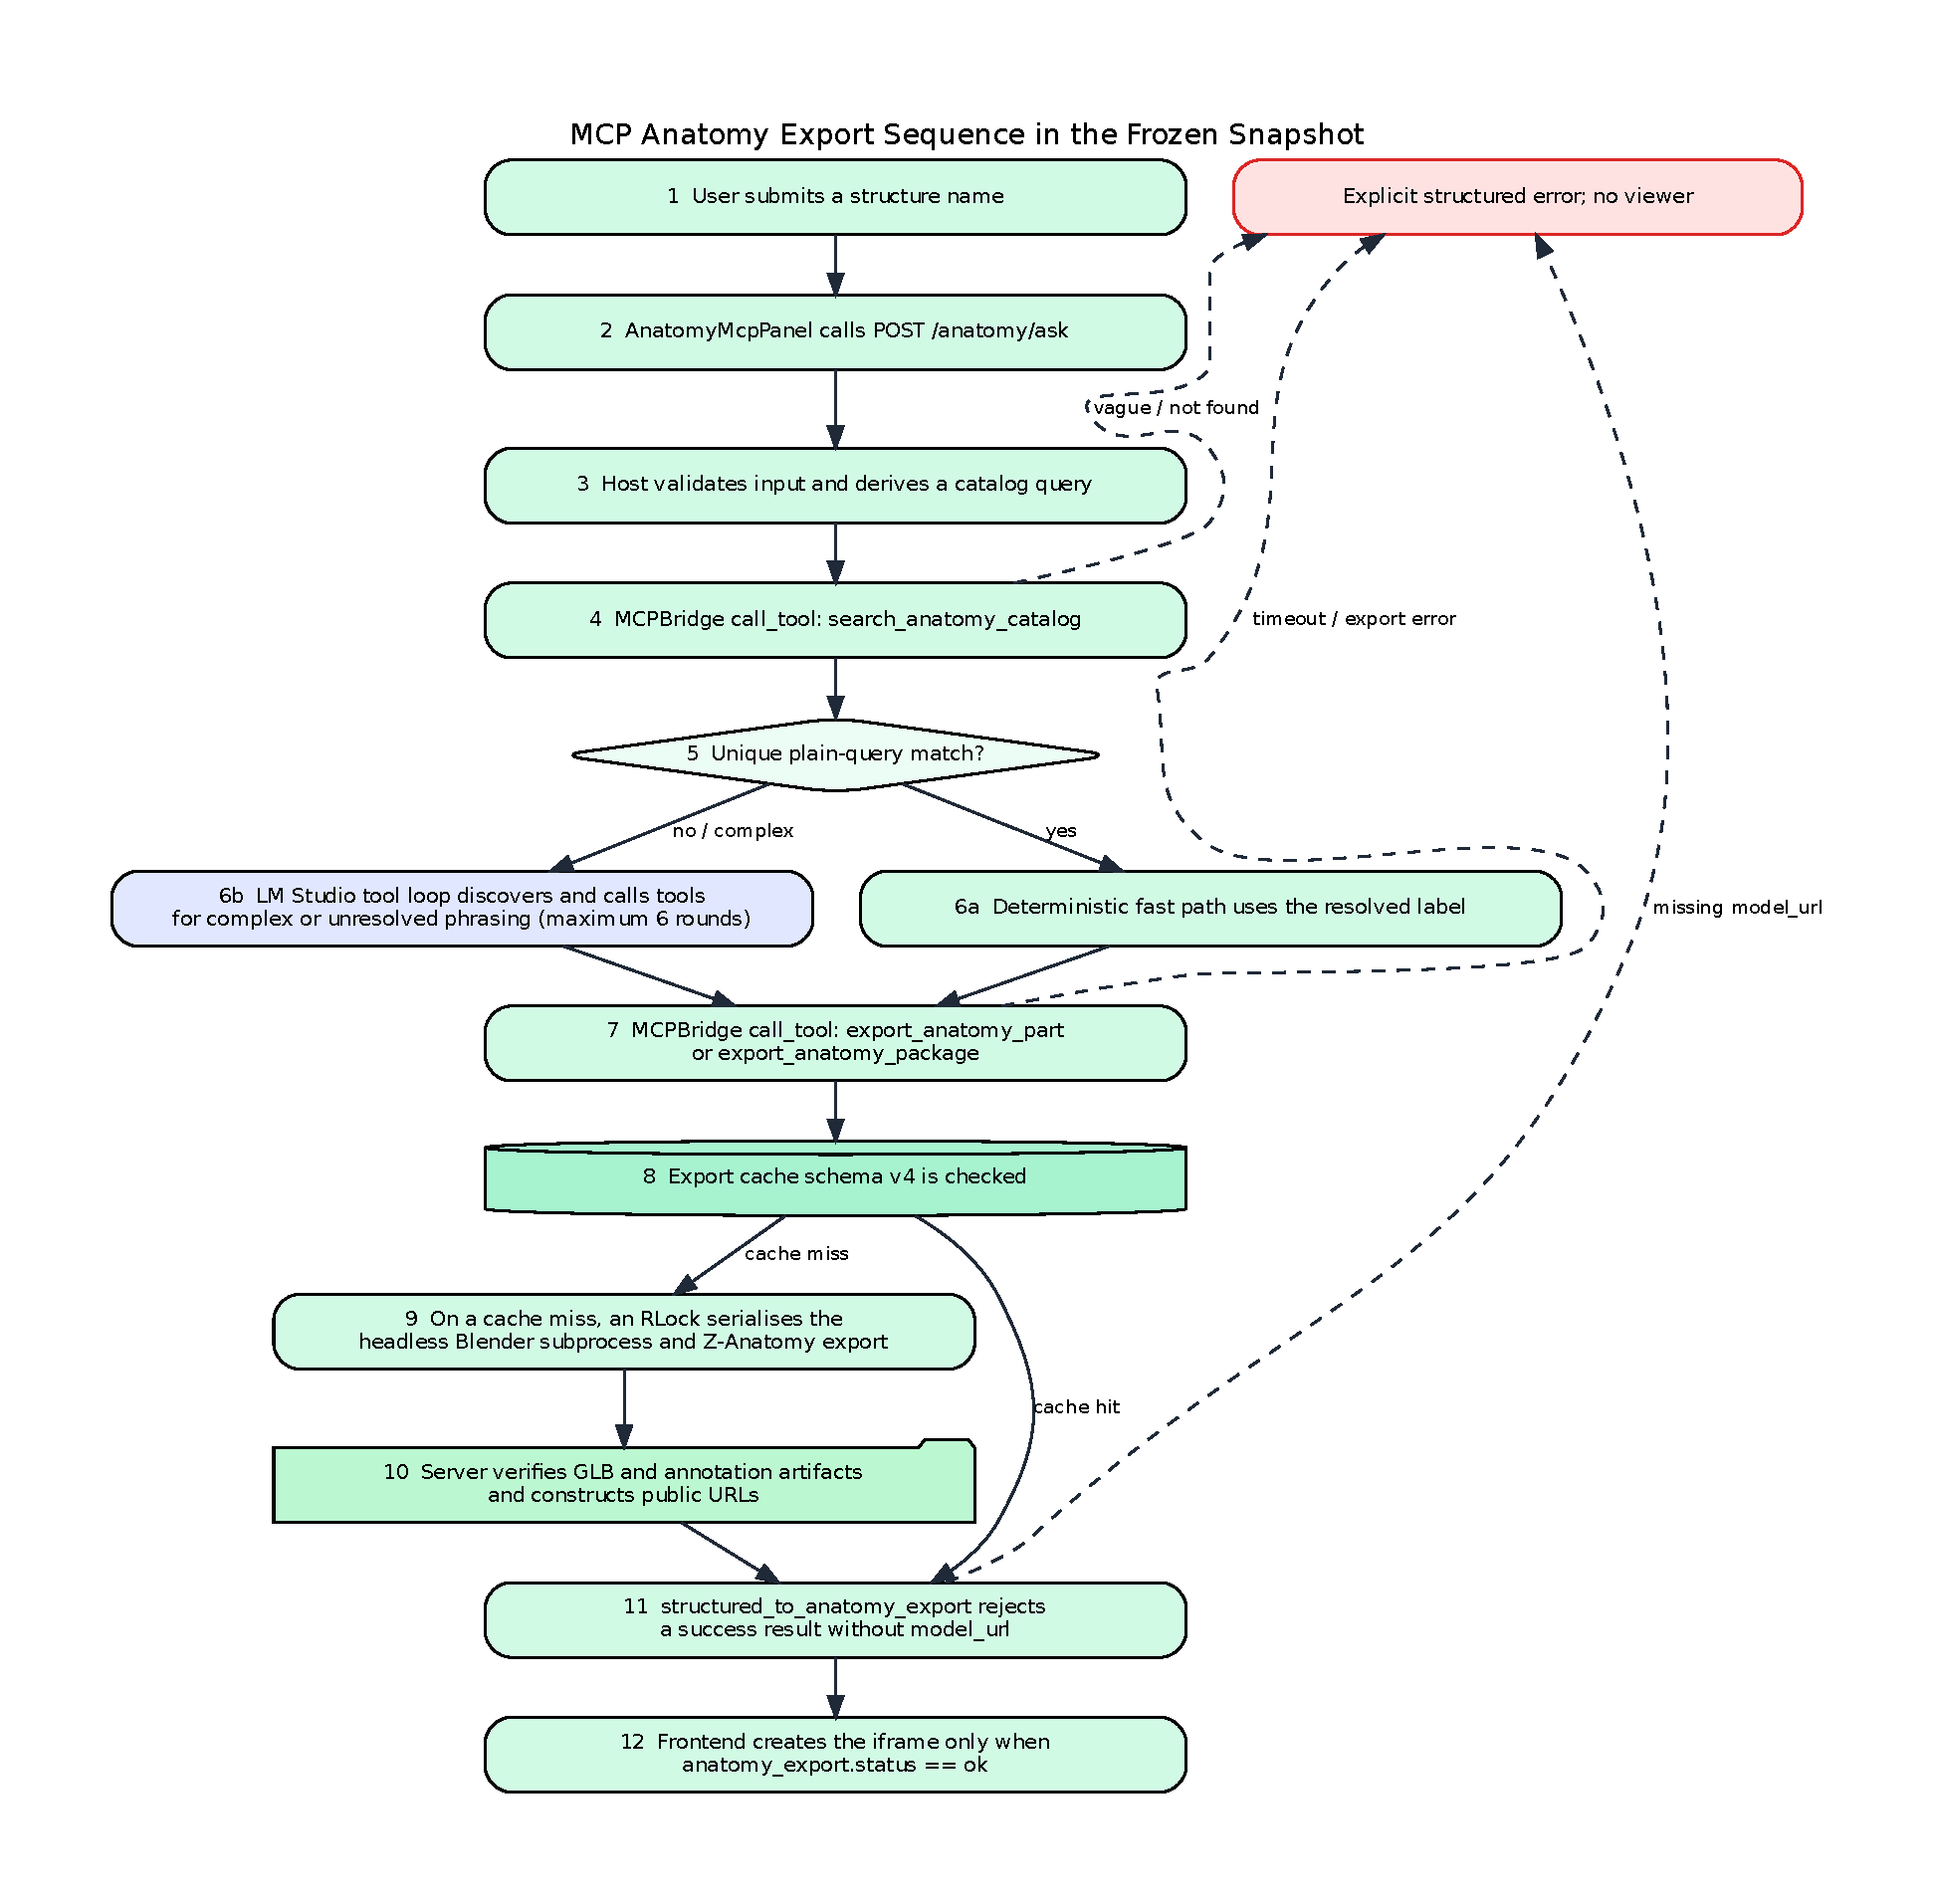
\includegraphics[width=\textwidth,height=0.68\textheight,keepaspectratio]{figures/rendered/mcp_runtime_sequence.pdf}
  \caption{MCP anatomy export sequence, including fast path, LLM tool loop, cache, Blender export, and explicit failure branches.}
  \label{fig:mcp-runtime-sequence}
\end{figure}

The host records \codepath{mcp_tools_used} and \codepath{mcp_tool_steps}. \codepath{structured_to_anatomy_export} creates a successful export object only if the tool result contains \codepath{model_url}. When configured, URL rewriting replaces development hosts with \codepath{PUBLIC_API_BASE}.

\section{FastMCP Server and Tool Schemas}
\label{sec:fastmcp-server}

The child process creates \codepath{FastMCP("Anatomy Blender MCP", json_response=True)} and exposes the tools in \cref{tab:mcp-tools}. Validation occurs before catalogue access or subprocess execution. Queries are limited to 80 characters and a conservative character set; Blender scripts and output paths are selected internally rather than supplied by the user.

\begin{table}[htbp]
  \centering
  \small
  \caption{FastMCP tools and structured responsibilities.}
  \label{tab:mcp-tools}
  \begin{tabularx}{\textwidth}{L{0.25\textwidth}L{0.28\textwidth}Y}
    \toprule
    Tool & Main input & Responsibility \\
    \midrule
    \codepath{search_anatomy_catalog} & Query and result limit & Validates and ranks exportable labels; returns laterality, match type, counts, suggestions, and catalogue metadata. \\
    \codepath{export_anatomy_part} & Part query, preview flag, optional region hint & Resolves one structure, serves a cache hit or runs Blender, verifies GLB/annotations, and returns public URLs. \\
    \codepath{export_anatomy_package} & Part query and package options & Exports large structures with a main GLB, annotations, manifest, optional materials, per-object files, preview, and timing metadata. \\
    \bottomrule
  \end{tabularx}
\end{table}

Explicit error codes distinguish vague, missing, ambiguous, configuration, timeout, subprocess, and artefact failures. The UI can handle these categories deterministically, and evaluation can score them separately. Arbitrary blend-file paths and Python programs are excluded from the schema.

\section{Geometry Catalogue and Structure Resolution}
\label{sec:catalog-resolution}

The bundled \codepath{exportable_catalog.json} uses schema version 1 and contains 6,075 entries: 555 collections and 5,520 objects. Its archive SHA-256 is \nolinkurl{a18357fb83bda6a1b9b3f329ead4be50dc2c26196200fe6358e73b51174d6350}. The recorded source path ends in \codepath{Startup.blend}, although the blend file is external. \codepath{build_exportable_catalog.py} retained entries with detected geometry. A complete evidence package still needs the exact Z-Anatomy release, licence, and blend-file hash \parencite{zanatomy}.

\codepath{query_validation.py} normalises natural-language input. The resolver checks exact and known aliases before token ranking and laterality rules. A phrase such as ``left femur'' can therefore resolve to \codepath{Femur.l} when the result is unique. Ambiguous cases return candidates rather than silently selecting the first match.

If the exportable catalogue is missing, the resolver can fall back to \codepath{z_anatomy_index.json} and sets \codepath{resolver_source=raw_index}. This preserves older behaviour but weakens the geometry-proven assumption. Evaluation records should therefore include the resolver source.

\section{Blender Export, GLB, Annotations, and Three.js}
\label{sec:blender-viewer}

After resolution, the server selects a part or package exporter, creates unique output paths, and launches Blender in background factory-startup mode. The command includes the external blend path, exporter script, canonical label, and resolved objects or collections. Default timeouts are 300 seconds for a part and 900 seconds for a package.

The subprocess runs within a process-wide re-entrant lock. Standard input is disconnected from the MCP transport, and standard error is merged with standard output. The server parses the final JSON object from the exporter, checks the return code and \codepath{ok} field, and verifies the GLB and annotation files. Requested previews are checked as well. Public URLs are built only after these conditions pass.

Blender's glTF pipeline produces the exported model \parencite{blenderGltf}. GLB contains browser-compatible geometry and scene data; annotations remain in a separate JSON file. The Three.js viewer uses \codepath{GLTFLoader} and \codepath{OrbitControls}, frames the model from its bounds, adds lighting, and places labels at annotation anchors. A successful protocol exchange confirms the file path, not the anatomical correctness of the resolved geometry, transforms, or annotations.

\section{Locking, Caching, Health Checks, and Safe Errors}
\label{sec:reliability}

\codepath{\_BLENDER_EXPORT_LOCK = threading.RLock()} serialises Blender calls inside one MCP server process. That fits the target single-machine Windows setup but cannot coordinate several processes or machines. Scaling would require an inter-process or distributed mechanism.

Cache schema \codepath{v4} builds part keys from schema version, canonical label, match type, and preview mode; package keys also include package options. A hit is accepted only when GLB and annotation files exist and the annotation JSON contains a record. Tool results expose \codepath{cache_hit} for later comparison. Because the key omits hashes of the blend file, catalogue, and exporter scripts, those changes require a schema update or cache deletion.

\codepath{/anatomy/health} checks Blender, the source blend, indexes, the MCP import, and the stdio bridge. Catalogue presence is reported but not required by the current \codepath{ready} expression, so the endpoint may claim readiness even when search would fail. A stronger probe would require the exportable catalogue and a successful tool-list or search call.

The host rejects structured success without \codepath{model_url}, and the frontend opens the viewer only for \codepath{status == ok}. Tool errors stay explicit; text salvage is the weaker exception. Unit tests cover query validation, left-femur resolution, URL normalisation, mocked tool loops, and rejection of unverified export prose. They do not run the external Blender/Z-Anatomy stack. API-test collection during the audit also failed because \codepath{openai} was absent from the installed environment, exposing a packaging gap.

\section{API Contract Summary}
\label{sec:api-contracts}

\begin{table}[htbp]
  \centering
  \small
  \caption{Principal HTTP contracts in the frozen FastAPI application.}
  \label{tab:api-contracts}
  \begin{tabularx}{\textwidth}{L{0.23\textwidth}L{0.09\textwidth}L{0.27\textwidth}Y}
    \toprule
    Endpoint & Method & Request & Principal response \\
    \midrule
    \codepath{/upload-pdf/} & POST & Multipart \codepath{file} & Stage status, text ingestion, image extraction, and elapsed time. \\
    \codepath{/rag/ask} & POST & \codepath{question} & Answer, sources, images, grounding metadata, and optional legacy render fields. \\
    \codepath{/rag/experiment/ask} & POST & Question and log flag & Baseline/strict answers, sources, judge output, and debug fields. \\
    \codepath{/anatomy/health} & GET & None & Configuration and stdio readiness checks. \\
    \codepath{/anatomy/search} & GET & Query \codepath{q}, optional limit & Catalogue result, suggestions, or structured error. \\
    \codepath{/anatomy/ask} & POST & Message and language & Answer, \codepath{anatomy_export}, tool audit trail, mode, and error. \\
    \codepath{/anatomy/export} & POST & Part query and export options & Structured export result or error. \\
    \codepath{/debug/storage} & GET & None & Provider, bucket checks, and sample keys. \\
    \codepath{/images/all} & GET & None & Local image URL list. \\
    \codepath{/blender/generate-brain-3d} & POST & Legacy generation request & Asset/preview URLs or error. \\
    \bottomrule
  \end{tabularx}
\end{table}

The schemas preserve the mode boundary. \codepath{AskResponse} is document-oriented, whereas \codepath{AnatomyAskResult} carries a structured artefact and tool trace. Most frontend/backend drift occurs in the document contract.

\section{Configuration and Reproducibility}
\label{sec:configuration-reproducibility}

Requirements files, \codepath{package-lock.json}, Docker images, model identifiers, and repository commits provide partial version evidence. \Cref{tab:environment-versions} separates the audit HEAD, the hybrid-connection commit, the earlier dense-only inspection snapshot, and declared dependency values from information that depends on the final machine.

\small
\setlength{\tabcolsep}{3pt}
\begin{longtable}{L{0.23\textwidth}L{0.39\textwidth}L{0.29\textwidth}}
  \caption{Environment and version record for the audited implementation timeline.}
  \label{tab:environment-versions}\\
  \toprule
  Item & Repository-declared value & Final evidence status \\
  \midrule
  \endfirsthead
  \caption[]{Environment and version record (continued).}\\
  \toprule
  Item & Repository-declared value & Final evidence status \\
  \midrule
  \endhead
  \midrule
  \multicolumn{3}{r}{Continued on next page}\\
  \endfoot
  \bottomrule
  \endlastfoot
  Audit snapshot & \nolinkurl{d3a544d0b2202b1e068b648968a2ae17f871bfa8} & Thesis audit HEAD; not a claim that every dependency was frozen with P1. \\
  Hybrid-connection commit & \nolinkurl{5089fcc0182f86c71558ccce21b75ebcb18b06f4} (12 July 2026) & \codepath{HybridRetriever} wired into \codepath{MultimodalRAG}/\codepath{/rag/ask}; preferred P1 route. \\
  Historical dense-only snapshot & \nolinkurl{cb041d52787f469bbbe0434e9fc7690edc122afa} (27 June 2026) & Earlier inspection baseline only; not the final or July-evaluated implementation. \\
  Backend base & Python \codepath{3.11-slim} & Runtime patch version required. \\
  Next.js / React & Next.js \codepath{16.2.4}; React/ReactDOM \codepath{19.2.5} & Lock-file verified; Node.js version required. \\
  Embedding libraries & \codepath{sentence-transformers==2.7.0}; \codepath{transformers==4.41.2} & Declared; installed freeze required. \\
  Text model & \codepath{sentence-transformers/all-MiniLM-L6-v2} & Model revision/cache hash required. \\
  CLIP model & \codepath{clip-ViT-B-32} & Model revision/cache hash required. \\
  Torch / NumPy & \codepath{torch==2.2.2}; \codepath{numpy==1.26.4} & Declared. \\
  Chroma & \codepath{chromadb>=1.5.0}; LangChain Chroma unpinned & Exact installed versions required. \\
  RAG model & Groq \codepath{llama-3.1-8b-instant} & Provider revision/date required. \\
  MCP endpoint & \codepath{LLM_API_BASE}; default \codepath{http://127.0.0.1:1234/v1} & Environment-configurable. \\
  MCP model & \codepath{settings.llm_model = llama-3.1-8b-instant} & Runtime identifier must be verified. \\
  MCP SDK & \codepath{mcp[cli]>=1.27.1} in a separate requirements file & Installed version required. \\
  Blender & Local default references 5.1; legacy image installs 4.0.2 & Actual MCP binary/version required. \\
  Z-Anatomy & External \codepath{Startup.blend} & External asset; exact release and source-file hash were not archived with the evaluation \\
  Catalogue & Schema 1; 6,075 entries; SHA-256 \nolinkurl{a18357fb83bda6a1b9b3f329ead4be50dc2c26196200fe6358e73b51174d6350} & Archive verified. \\
  Storage & MinIO or Supabase selected by environment & Provider, bucket policy, and URL expiry required. \\
  Hardware / OS & Not recorded & Hardware details were not archived; evaluation date was 12 July 2026 \\
\end{longtable}
\normalsize

The declared environment has three dependency gaps. \codepath{anatomy_mcp_chat.py} imports \codepath{openai.AsyncOpenAI}, but the root requirements omit \codepath{openai}. \codepath{HybridRetriever} depends on undeclared \codepath{rank_bm25}. The MCP SDK appears only in \codepath{anatomy_mcp/requirements.txt}, while the backend Dockerfile installs the root requirements. Additional installation is therefore required before the backend image can be assumed to run the MCP path.

Model configuration drifts as well. \codepath{.env.example} documents \codepath{LLM_MODEL=qwen2.5-7b-instruct-1m}, while \codepath{Settings.llm_model} is a constant shared by Groq synthesis and the LM Studio tool loop. Separate RAG and MCP variables would make the resolved runtime easier to record and test.

A reproducible release still requires corpus hashes, a deterministic index build, prompt versions, object-storage settings, Blender and Z-Anatomy hashes, the catalogue hash, hardware, operating system, and evaluation date. The repository supports a detailed source-level architecture account, but the missing runtime record prevents a claim of fully reproducible deployment.

\section{Chapter Summary}
\label{sec:implementation-summary}

The archive contains a substantial implementation: PDF ingestion, MiniLM--Chroma and BM25 hybrid retrieval, CLIP figure search, duplicate filtering, type-dependent context selection, local or cloud generation, object-storage URLs, an MCP stdio boundary, catalogue resolution, locked and cached Blender export, artefact checks, and a guarded Three.js viewer. The MCP route is close to the documented architecture. The document route is hybrid-preferred after \texttt{5089fcc}, while world-knowledge consent enforcement and post-generation citation verification remain incomplete on \codepath{/rag/ask}. The evaluation and conclusions therefore follow the verified active route rather than every module present in the repository.
